\chapter{Exemplary Evaluation of Results}
\label{cha:results}
To familiarize with the potential of Visual Bicycle Counter, I have prepared an exemplary interpretation of the Counter's data. I have been collecting video files from two street cameras --- one near ICE Krakow Congress Centre and second on Lema Street. For ICE Krakow Congress Centre I have chosen two months --- June and September, where pandemic restrictions were less strict and that had as similar weather conditions as possible. For Lema Street I have chosen one week of July (6th--13th) and October (5th--12th), to show differences in bicycle traffic before and after modernization of bike road. Figure \ref{fig:map} shows those cameras' position on map of Krakow.
\begin{figure}[H]
    \centering
    \resizebox{\textwidth}{!}{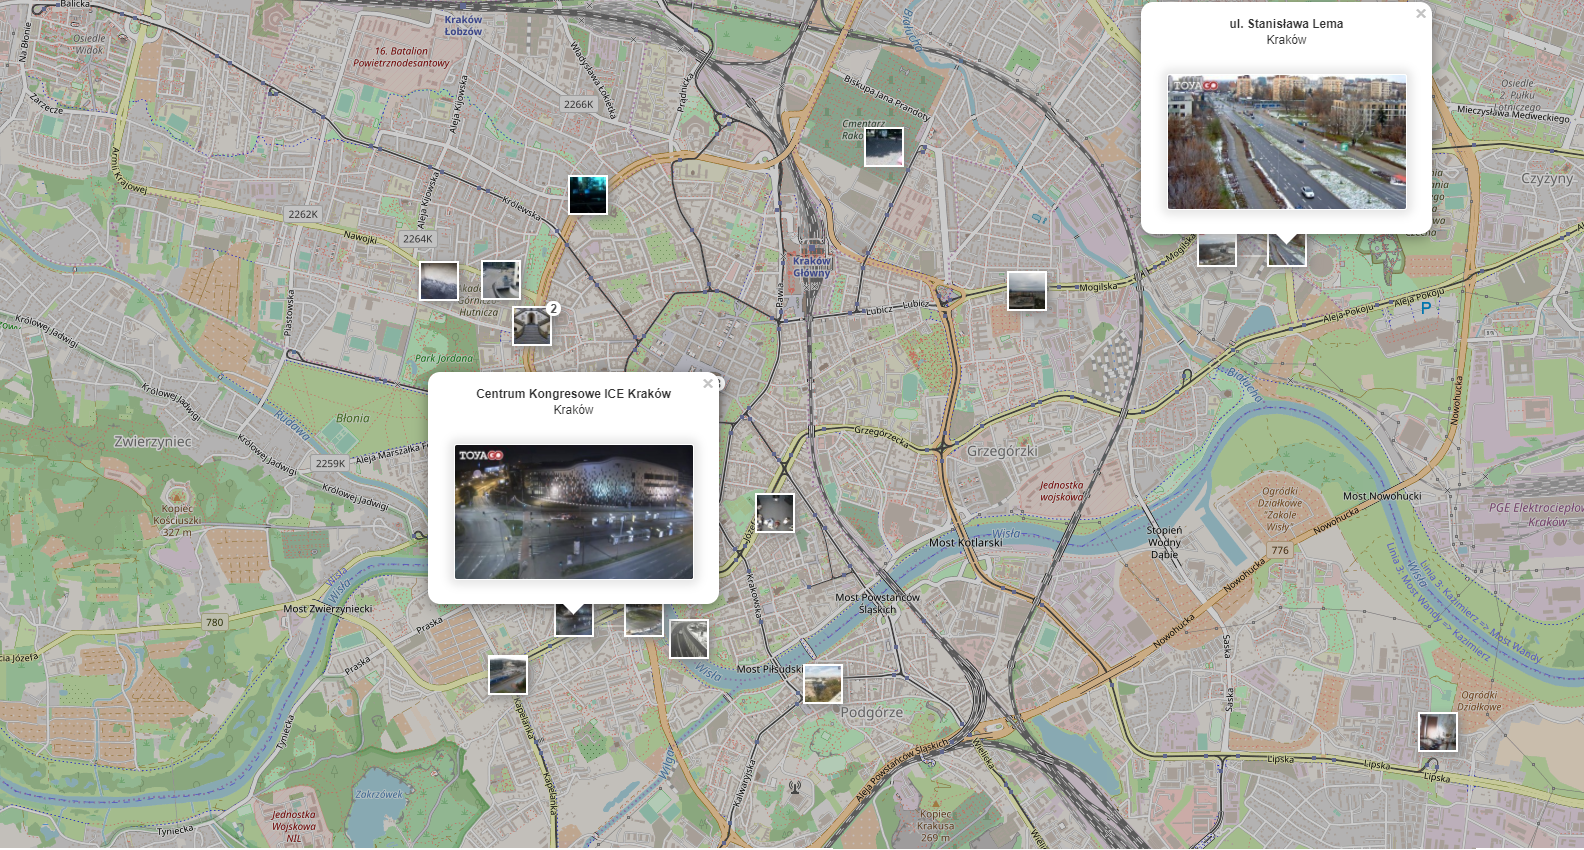
\includegraphics{images/map}}
    \caption{Position of cameras comes from "worldcam.pl" website \cite{mapa}}
    \label{fig:map}
\end{figure}

\section{Data Collected From Camera Near Ice Krakow Congress Centre}
\label{sec:ice}
For first example I had chosen video files collected between 8:30 AM and 6:30 PM on June and September on bike road near ICE Krakow Congress Centre and performed inference on them. Tables \ref{tab:iceCountJune} and \ref{tab:iceCountSeptember} shows collected cyclists count. Table \ref{tab:iceDaily} aggregates this data to show number of cyclists per day of both months. All collected raw data is also accessible on repositories \cite{repo}, \cite{repoSL}.
\begin{table}[H]
\centering
\resizebox{\textwidth}{!}{
\begin{tabular}{|r|r|r|r|r|r|r|r|r|r|r|}
\hline
\multicolumn{1}{|l|}{} & \multicolumn{10}{c|}{Cyclist count throughout the day (June)}                                                                                                                                                                                                                                                                                            \\ \hline
\multicolumn{1}{|l|}{} & \multicolumn{1}{l|}{8:30--9:30} & \multicolumn{1}{l|}{9:30--10:30} & \multicolumn{1}{l|}{10:30--11:30} & \multicolumn{1}{l|}{11:30--12:30} & \multicolumn{1}{l|}{12:30--13:30} & \multicolumn{1}{l|}{13:30--14:30} & \multicolumn{1}{l|}{14:30--15:30} & \multicolumn{1}{l|}{15:30--16:30} & \multicolumn{1}{l|}{16:30--17:30} & \multicolumn{1}{l|}{17:30--18:30} \\ \hline
1.                     & 307                            & 404                             & 308                              & 302                              & 428                              & 221                              & 98                               & 235                              & 207                              & 239                              \\ \hline
2.                     & 357                            & 313                             & 291                              & 196                              & 214                              & 198                              & 332                              & 141                              & 60                               & 82                               \\ \hline
3.                     & 148                            & 337                             & 479                              & 47                               & 390                              & 330                              & 401                              & 132                              & 78                               & 374                              \\ \hline
4.                     & 364                            & 62                              & 370                              & 288                              & 301                              & 510                              & 467                              & 110                              & 420                              & 103                              \\ \hline
5.                     & 82                             & 45                              & 98                               & 237                              & 138                              & 127                              & 170                              & 50                               & 152                              & 199                              \\ \hline
6.                     & 472                            & 210                             & 120                              & 417                              & 32                               & 306                              & 492                              & 377                              & 265                              & 572                              \\ \hline
7.                     & 251                            & 250                             & 142                              & 372                              & 38                               & 352                              & 225                              & 62                               & 119                              & 83                               \\ \hline
8.                     & 56                             & 124                             & 134                              & 46                               & 71                               & 148                              & 41                               & 389                              & 440                              & 130                              \\ \hline
9.                     & 261                            & 66                              & 154                              & 397                              & 240                              & 73                               & 298                              & 371                              & 103                              & 214                              \\ \hline
10.                    & 179                            & 85                              & 374                              & 96                               & 243                              & 182                              & 52                               & 187                              & 150                              & 328                              \\ \hline
11.                    & 259                            & 244                             & 333                              & 251                              & 321                              & 326                              & 135                              & 190                              & 205                              & 121                              \\ \hline
12.                    & 364                            & 225                             & 282                              & 169                              & 164                              & 320                              & 117                              & 153                              & 168                              & 91                               \\ \hline
13.                    & 273                            & 72                              & 108                              & 265                              & 301                              & 56                               & 126                              & 298                              & 275                              & 343                              \\ \hline
14.                    & 140                            & 95                              & 124                              & 55                               & 171                              & 237                              & 147                              & 159                              & 327                              & 364                              \\ \hline
15.                    & 386                            & 269                             & 224                              & 374                              & 137                              & 139                              & 307                              & 98                               & 323                              & 419                              \\ \hline
16.                    & 246                            & 85                              & 51                               & 337                              & 281                              & 172                              & 87                               & 359                              & 275                              & 74                               \\ \hline
17.                    & 73                             & 197                             & 176                              & 98                               & 275                              & 49                               & 400                              & 84                               & 212                              & 110                              \\ \hline
18.                    & 88                             & 198                             & 202                              & 344                              & 110                              & 143                              & 289                              & 77                               & 321                              & 272                              \\ \hline
19.                    & 85                             & 23                              & 266                              & 192                              & 79                               & 171                              & 217                              & 270                              & 34                               & 235                              \\ \hline
20.                    & 269                            & 44                              & 148                              & 305                              & 22                               & 296                              & 110                              & 192                              & 144                              & 222                              \\ \hline
21.                    & 123                            & 105                             & 57                               & 101                              & 174                              & 15                               & 27                               & 52                               & 102                              & 85                               \\ \hline
22.                    & 62                             & 72                              & 143                              & 195                              & 10                               & 122                              & 87                               & 173                              & 137                              & 28                               \\ \hline
23.                    & 382                            & 136                             & 485                              & 435                              & 315                              & 194                              & 264                              & 535                              & 273                              & 320                              \\ \hline
24.                    & 183                            & 89                              & 342                              & 280                              & 164                              & 92                               & 364                              & 222                              & 292                              & 266                              \\ \hline
25.                    & 297                            & 423                             & 340                              & 41                               & 381                              & 191                              & 48                               & 417                              & 355                              & 470                              \\ \hline
26.                    & 471                            & 137                             & 268                              & 115                              & 304                              & 107                              & 86                               & 364                              & 210                              & 243                              \\ \hline
27.                    & 70                             & 109                             & 363                              & 109                              & 207                              & 176                              & 242                              & 314                              & 212                              & 395                              \\ \hline
28.                    & 197                            & 331                             & 111                              & 158                              & 264                              & 261                              & 485                              & 425                              & 109                              & 410                              \\ \hline
29.                    & 154                            & 236                             & 26                               & 252                              & 103                              & 226                              & 214                              & 189                              & 60                               & 141                              \\ \hline
30.                    & 362                            & 108                             & 404                              & 416                              & 413                              & 517                              & 494                              & 351                              & 388                              & 92                               \\ \hline
\end{tabular}}
\caption{Cyclists count collected from street camera at bike road near ICE Krakow Congress Centre - June}
\label{tab:iceCountJune}
\end{table}
\begin{table}[H]
\centering
\resizebox{\textwidth}{!}{
\begin{tabular}{|r|r|r|r|r|r|r|r|r|r|r|}
\hline
\multicolumn{1}{|l|}{} & \multicolumn{10}{c|}{Cyclist count throughout the day (September)}                                                                                                                                                                                                                                                                                       \\ \hline
\multicolumn{1}{|l|}{} & \multicolumn{1}{l|}{8:30--9:30} & \multicolumn{1}{l|}{9:30--10:30} & \multicolumn{1}{l|}{10:30--11:30} & \multicolumn{1}{l|}{11:30--12:30} & \multicolumn{1}{l|}{12:30--13:30} & \multicolumn{1}{l|}{13:30--14:30} & \multicolumn{1}{l|}{14:30--15:30} & \multicolumn{1}{l|}{15:30--16:30} & \multicolumn{1}{l|}{16:30--17:30} & \multicolumn{1}{l|}{17:30--18:30} \\ \hline
1.                     & 78                             & 138                             & 71                               & 126                              & 174                              & 153                              & 157                              & 10                               & 73                               & 36                               \\ \hline
2.                     & 326                            & 294                             & 288                              & 127                              & 211                              & 93                               & 105                              & 461                              & 258                              & 110                              \\ \hline
3.                     & 540                            & 400                             & 237                              & 353                              & 102                              & 154                              & 340                              & 323                              & 439                              & 270                              \\ \hline
4.                     & 128                            & 106                             & 278                              & 359                              & 550                              & 161                              & 88                               & 305                              & 144                              & 619                              \\ \hline
5.                     & 284                            & 210                             & 588                              & 302                              & 188                              & 481                              & 317                              & 127                              & 109                              & 182                              \\ \hline
6.                     & 147                            & 74                              & 58                               & 54                               & 121                              & 57                               & 10                               & 164                              & 159                              & 79                               \\ \hline
7.                     & 222                            & 62                              & 183                              & 78                               & 216                              & 24                               & 180                              & 121                              & 215                              & 49                               \\ \hline
8.                     & 297                            & 498                             & 262                              & 254                              & 243                              & 422                              & 476                              & 467                              & 128                              & 56                               \\ \hline
9.                     & 439                            & 571                             & 13                               & 378                              & 531                              & 535                              & 242                              & 164                              & 421                              & 146                              \\ \hline
10.                    & 454                            & 420                             & 413                              & 255                              & 142                              & 291                              & 117                              & 257                              & 80                               & 99                               \\ \hline
11.                    & 58                             & 252                             & 126                              & 245                              & 477                              & 438                              & 213                              & 441                              & 295                              & 412                              \\ \hline
12.                    & 221                            & 361                             & 403                              & 220                              & 324                              & 217                              & 255                              & 47                               & 231                              & 367                              \\ \hline
13.                    & 201                            & 448                             & 331                              & 225                              & 94                               & 240                              & 436                              & 326                              & 283                              & 171                              \\ \hline
14.                    & 556                            & 256                             & 180                              & 376                              & 422                              & 154                              & 545                              & 64                               & 399                              & 306                              \\ \hline
15.                    & 485                            & 354                             & 539                              & 100                              & 48                               & 112                              & 442                              & 440                              & 633                              & 271                              \\ \hline
16.                    & 108                            & 306                             & 603                              & 404                              & 490                              & 127                              & 606                              & 122                              & 383                              & 374                              \\ \hline
17.                    & 555                            & 58                              & 268                              & 488                              & 125                              & 87                               & 35                               & 251                              & 241                              & 309                              \\ \hline
18.                    & 281                            & 387                             & 263                              & 413                              & 258                              & 186                              & 262                              & 120                              & 135                              & 117                              \\ \hline
19.                    & 155                            & 184                             & 138                              & 280                              & 257                              & 106                              & 164                              & 300                              & 224                              & 326                              \\ \hline
20.                    & 424                            & 331                             & 406                              & 279                              & 17                               & 372                              & 119                              & 23                               & 108                              & 58                               \\ \hline
21.                    & 227                            & 375                             & 202                              & 365                              & 131                              & 394                              & 184                              & 229                              & 381                              & 307                              \\ \hline
22.                    & 282                            & 302                             & 273                              & 458                              & 433                              & 439                              & 116                              & 449                              & 129                              & 360                              \\ \hline
23.                    & 393                            & 304                             & 274                              & 283                              & 378                              & 413                              & 284                              & 343                              & 168                              & 111                              \\ \hline
24.                    & 419                            & 525                             & 525                              & 146                              & 89                               & 325                              & 508                              & 129                              & 120                              & 45                               \\ \hline
25.                    & 101                            & 168                             & 258                              & 381                              & 353                              & 191                              & 59                               & 384                              & 114                              & 27                               \\ \hline
26.                    & 143                            & 152                             & 11                               & 186                              & 74                               & 40                               & 9                                & 136                              & 36                               & 180                              \\ \hline
27.                    & 112                            & 26                              & 116                              & 41                               & 169                              & 176                              & 86                               & 116                              & 11                               & 249                              \\ \hline
28.                    & 139                            & 227                             & 156                              & 73                               & 105                              & 248                              & 48                               & 5                                & 22                               & 244                              \\ \hline
29.                    & 234                            & 207                             & 168                              & 187                              & 201                              & 160                              & 246                              & 41                               & 76                               & 218                              \\ \hline
30.                    & 105                            & 62                              & 72                               & 12                               & 78                               & 105                              & 38                               & 42                               & 95                               & 117                              \\ \hline
\end{tabular}}
\caption{Cyclists count collected from street camera at bike road near ICE Krakow Congress Centre --- September}
\label{tab:iceCountSeptember}
\end{table}
\begin{table}[H]
\centering
\begin{tabular}{|r|r|r|}
\hline
\multicolumn{1}{|l|}{}                 & \multicolumn{2}{c|}{Cyclist count}                         \\ \hline
\multicolumn{1}{|l|}{Day of the month} & \multicolumn{1}{l|}{June} & \multicolumn{1}{l|}{September} \\ \hline
1                                      & 2749                      & 1016                           \\ \hline
2                                      & 2184                      & 2273                           \\ \hline
3                                      & 2716                      & 3158                           \\ \hline
4                                      & 2995                      & 2738                           \\ \hline
5                                      & 1298                      & 2788                           \\ \hline
6                                      & 3263                      & 923                            \\ \hline
7                                      & 1894                      & 1350                           \\ \hline
8                                      & 1579                      & 3103                           \\ \hline
9                                      & 2177                      & 3440                           \\ \hline
10                                     & 1876                      & 2528                           \\ \hline
11                                     & 2385                      & 2957                           \\ \hline
12                                     & 2053                      & 2646                           \\ \hline
13                                     & 2117                      & 2755                           \\ \hline
14                                     & 1819                      & 3258                           \\ \hline
15                                     & 2676                      & 3424                           \\ \hline
16                                     & 1967                      & 3523                           \\ \hline
17                                     & 1674                      & 2417                           \\ \hline
18                                     & 2044                      & 2422                           \\ \hline
19                                     & 1572                      & 2134                           \\ \hline
20                                     & 1752                      & 2137                           \\ \hline
21                                     & 841                       & 2795                           \\ \hline
22                                     & 1029                      & 3241                           \\ \hline
23                                     & 3339                      & 2951                           \\ \hline
24                                     & 2294                      & 2831                           \\ \hline
25                                     & 2963                      & 2036                           \\ \hline
26                                     & 2305                      & 967                            \\ \hline
27                                     & 2197                      & 1102                           \\ \hline
28                                     & 2751                      & 1267                           \\ \hline
29                                     & 1601                      & 1738                           \\ \hline
30                                     & 3545                      & 726                            \\ \hline
\multicolumn{1}{|l|}{Sum}              & 65655                     & 70644                          \\ \hline
\end{tabular}
\caption{Daily cyclists count collected from street camera near ICE Krakow Conference Center (sum of numbers for each day from Tables \ref{tab:iceCountJune} and \ref{tab:iceCountSeptember}).}
\label{tab:iceDaily}
\end{table}

I have aggregated this data and put it on a graphs. Figure \ref{fig:graph2} shows graphical comparison of mean cyclists count during the day basing on data data from Tables \ref{tab:iceCountJune} and \ref{tab:iceCountSeptember} (monthly mean value for each hour).
\begin{figure}[H]
    \centering
    \resizebox{\textwidth}{!}{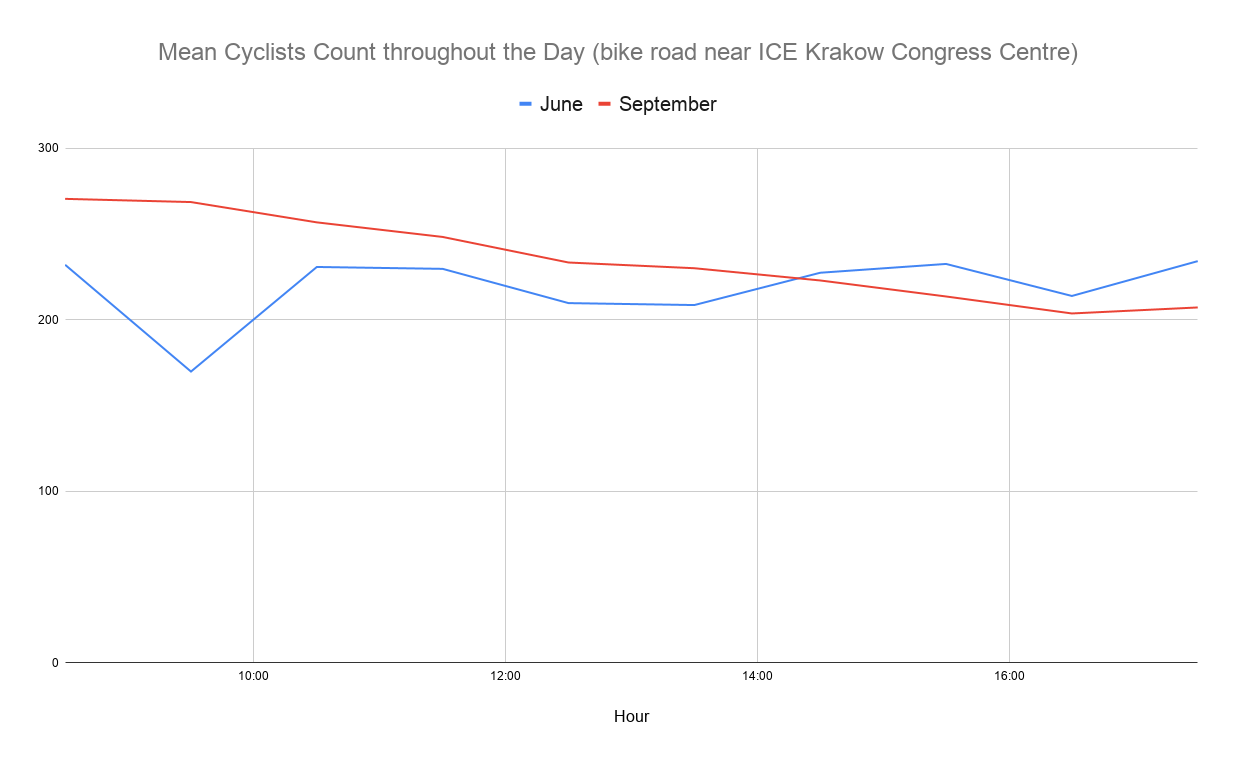
\includegraphics{images/graph4}}
    \caption{Cyclists count during the day --- June to September comparison (bike road near ICE Krakow Congress Centre)}
    \label{fig:graph4}
\end{figure}
Figures \ref{fig:graph2} and \ref{fig:graph9} shows data from Table \ref{tab:iceDaily} for easier comparison of results.
\begin{figure}[H]
    \centering
    \resizebox{\textwidth}{!}{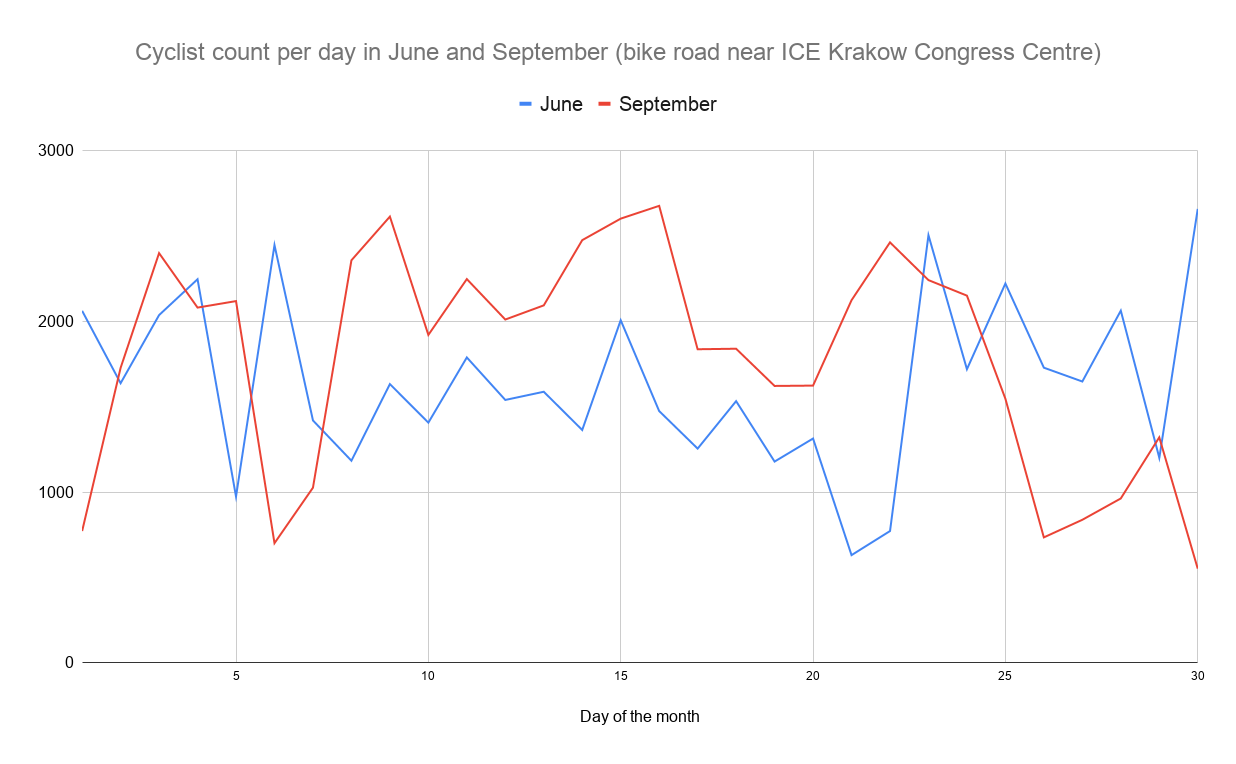
\includegraphics{images/graph2}}
    \caption{Cyclists count during the month --- June to September comparison (bike road near ICE Krakow Congress Centre)}
    \label{fig:graph2}
\end{figure}
\begin{figure}[H]
    \centering
    \resizebox{\textwidth}{!}{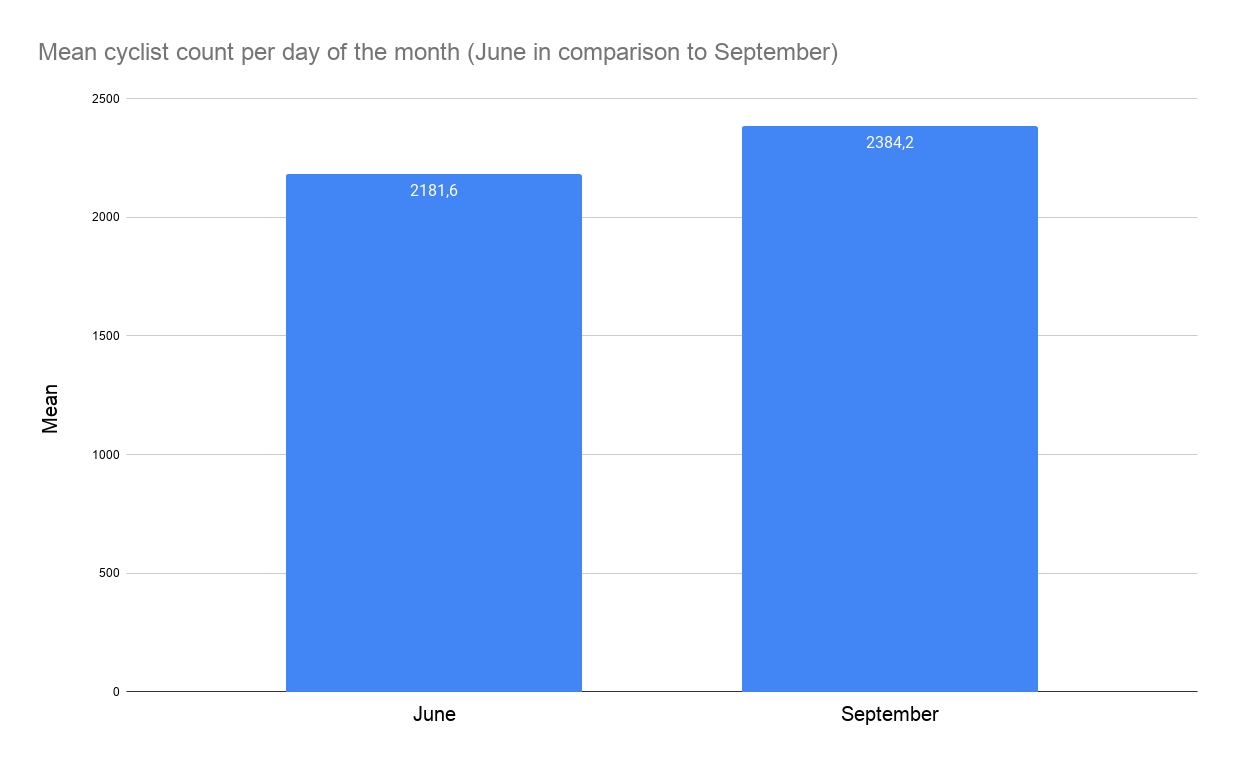
\includegraphics{images/graph9}}
    \caption{Mean cyclists count per day of the month --- June to September comparison (bike road near ICE Krakow Congress Centre)}
    \label{fig:graph9}
\end{figure}

Figures \ref{fig:graph7}, \ref{fig:graph8} shows data aggregated to compare how many cyclists rode near ICE per day of the week in June and October (mean value). We can analyse this data on various levels. For example, why was those numbers so irregular during the week in June, but in September in the other hand it was more regular --- higher on work days, but dropping at weekends. This can indicate, that maybe in September more people use bikes to get to their school or work, when in June maybe people use their bike more as a hobby than as a mean of transport. 
\begin{figure}[H]
    \centering
    \resizebox{\textwidth}{!}{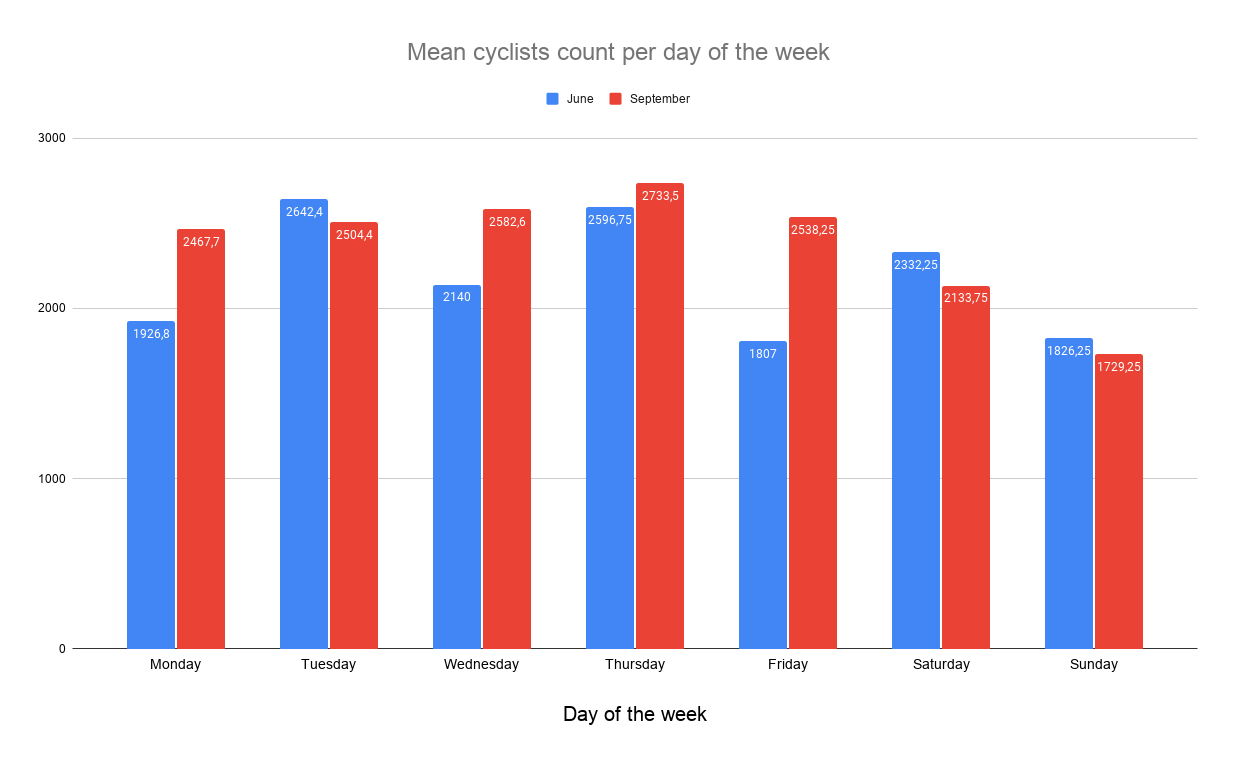
\includegraphics{images/graph7}}
    \caption{Mean cyclists count per day of the week --- June to September comparison (bike road near ICE Krakow Congress Centre)}
    \label{fig:graph7}
\end{figure}
\begin{figure}[H]
    \centering
    \resizebox{\textwidth}{!}{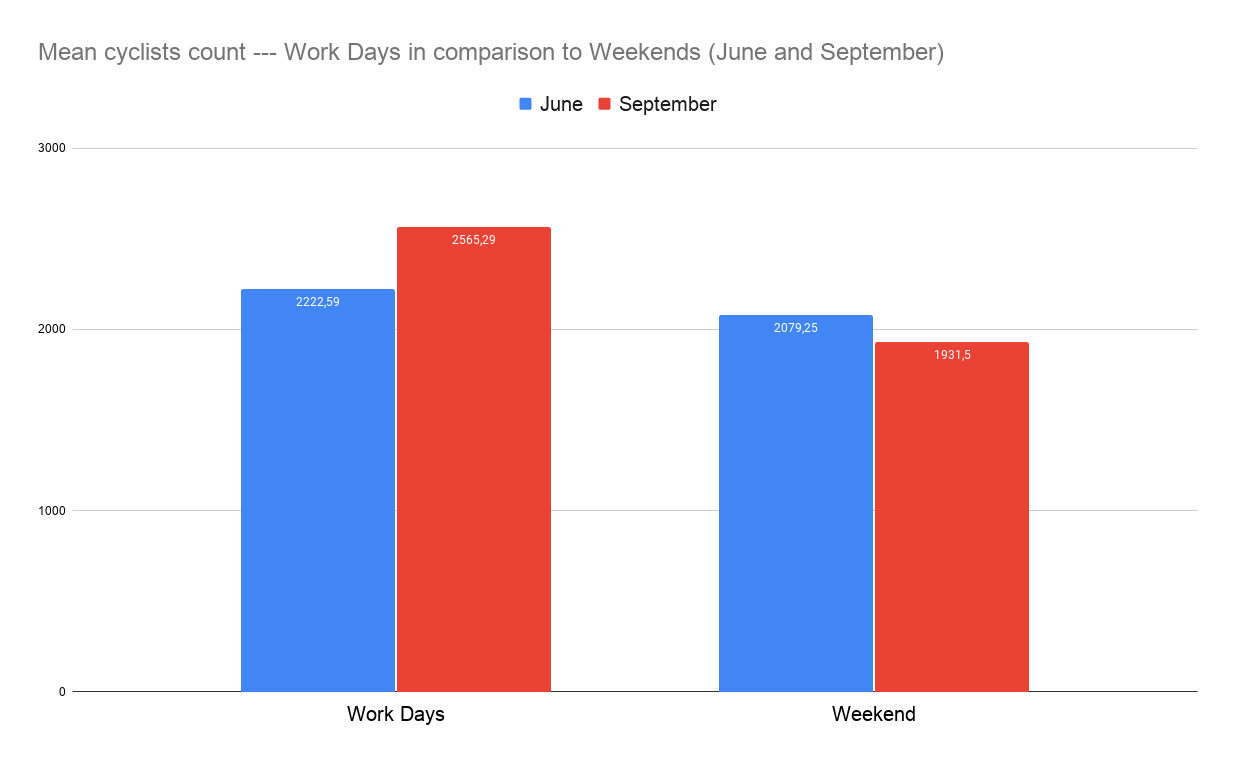
\includegraphics{images/graph8}}
    \caption{Mean cyclists count per day of the week --- June to September comparison of Work Days and Weekends (bike road near ICE Krakow Congress Centre)}
    \label{fig:graph8}
\end{figure}
This simple example provides important information on how bicycle traffic changes on different months of the year. It shows if it grows or not. Various conclusions can be drawn. For example in Figure \ref{fig:graph4} we can see that even though in September number of cyclists is higher that in June on early hours, it drops in later hours. After deeper analysis of different conditions those information can become a signal that maybe street lighting needs to be improved, considering that September is still quite warm month. It could be one of the ways to plan local government's projects.
\section{Data Collected From Camera at Lema Street}
\label{sec:lema}
Second example shows different interpretation of similar data collected from camera on Lema Street where bike road was modernized. Table \ref{tab:lemaCount} show cyclists count during days of random week from July (before modernization) and October (after modernization). Table \ref{tab:lemaSum} shows summed numbers from Table \ref{tab:lemaCount}. 
\begin{table}[H]
    \centering
    \resizebox{\textwidth}{!}{
    \begin{tabular}{|r|r|r|r|r|r|r|r|r|r|r|r|r|r|}
\hline
\multicolumn{7}{|c|}{Cyclists count throughout the day --- July}                    & \multicolumn{7}{c|}{Cyclists count throughout the day --- October}                     \\ \hline
09:45:00 & 10:45:00 & 11:45:00 & 12:45:00 & 13:45:00 & 14:45:00 & 15:45:00 & 09:45:00 & 10:45:00 & 11:45:00 & 12:45:00 & 13:45:00 & 14:45:00 & 15:45:00 \\ \hline
20       & 53       & 68       & 118      & 178      & 210      & 190      & 232      & 255      & 249      & 263      & 260      & 192      & 178      \\ \hline
229      & 261      & 180      & 386      & 210      & 305      & 436      & 419      & 291      & 311      & 424      & 353      & 216      & 259      \\ \hline
117      & 277      & 505      & 471      & 11       & 98       & 397      & 138      & 98       & 188      & 318      & 157      & 314      & 339      \\ \hline
118      & 385      & 92       & 315      & 350      & 121      & 290      & 390      & 499      & 271      & 373      & 104      & 212      & 61       \\ \hline
518      & 219      & 319      & 50       & 443      & 344      & 336      & 436      & 362      & 343      & 232      & 64       & 229      & 467      \\ \hline
293      & 179      & 130      & 171      & 49       & 27       & 12       & 485      & 519      & 331      & 242      & 118      & 97       & 41       \\ \hline
315      & 184      & 153      & 360      & 482      & 496      & 521      & 54       & 307      & 83       & 47       & 77       & 161      & 282      \\ \hline
\end{tabular}}
    \caption{Cyclist count during the day --- week from July to week from October comparison (bike road on Lema Street)}
    \label{tab:lemaCount}
\end{table}
\begin{table}[H]
    \centering
    \begin{tabular}{|r|r|r|}
\hline
\multicolumn{1}{|l|}{}                & \multicolumn{2}{c|}{Cyclists count}                                \\ \hline
\multicolumn{1}{|l|}{Day of the week} & \multicolumn{1}{l|}{6--13 July} & \multicolumn{1}{l|}{5--12 October} \\ \hline
1                                     & 837                            & 1629                              \\ \hline
2                                     & 2007                           & 2273                              \\ \hline
3                                     & 1876                           & 1552                              \\ \hline
4                                     & 1671                           & 1910                              \\ \hline
5                                     & 2229                           & 2133                              \\ \hline
6                                     & 861                            & 1833                              \\ \hline
7                                     & 2511                           & 1011                              \\ \hline
\end{tabular}
    \caption{Daily cyclists count collected from street camera on Lema Street (sum of numbers for each day from Table \ref{tab:lemaCount})}
    \label{tab:lemaSum}
\end{table}
Aggregation of this data for putting it on graphs like in first example:
\begin{figure}[H]
    \centering
    \resizebox{\textwidth}{!}{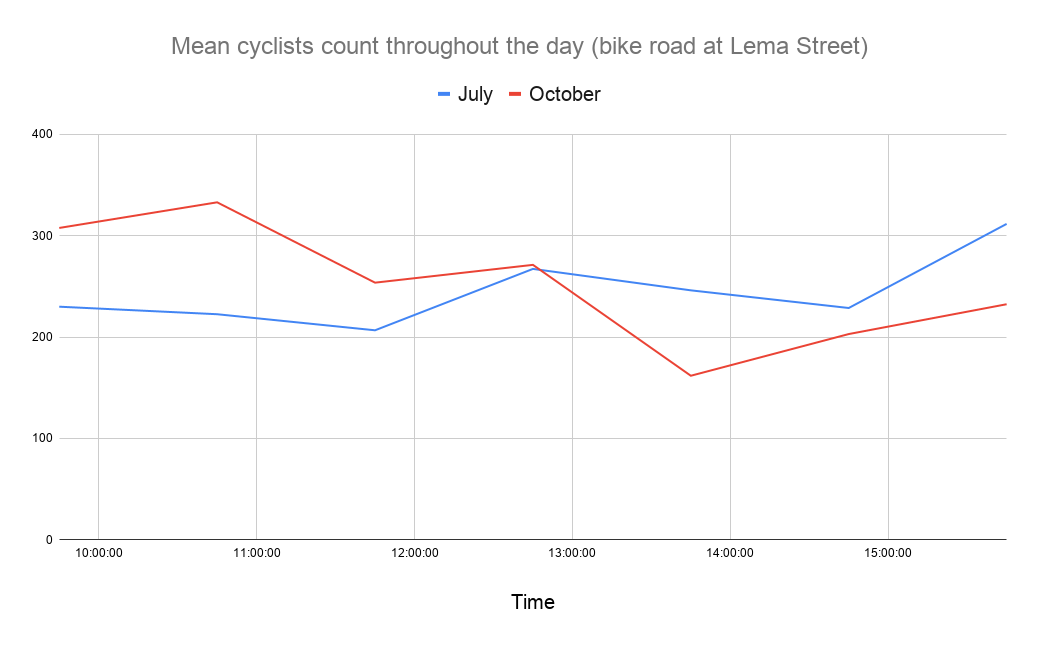
\includegraphics{images/graph6}}
    \caption{Weekly mean cyclists count on Lema Street for each hour --- July to October comparison}
    \label{fig:lemaCount}
\end{figure}
\begin{figure}[H]
    \centering
    \resizebox{\textwidth}{!}{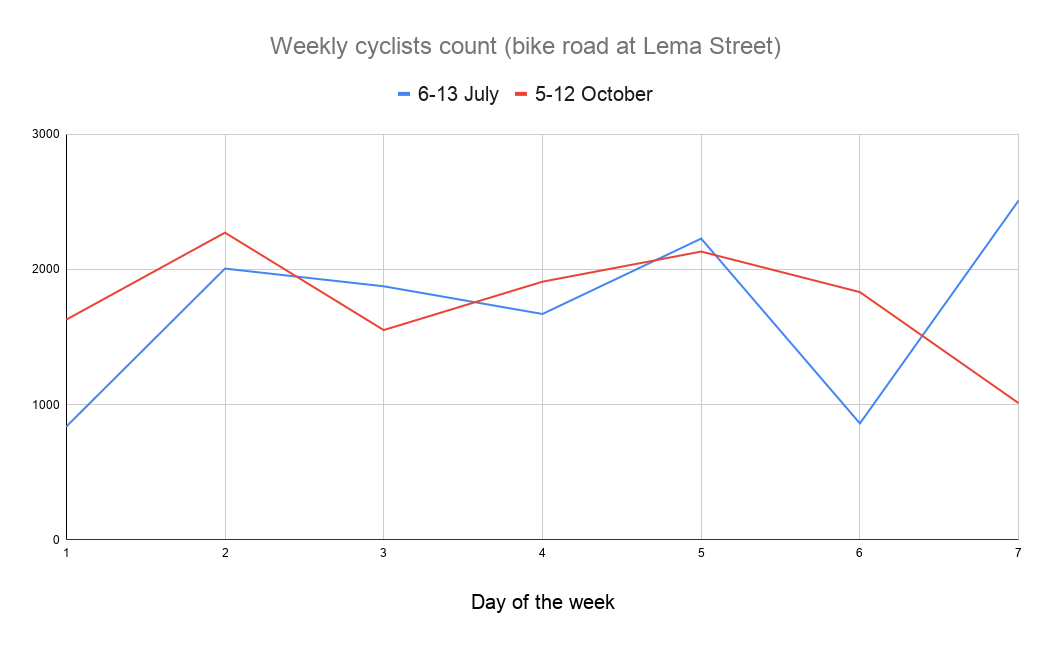
\includegraphics{images/graph5}}
    \caption{Cyclists count on Lema Street during chosen week --- July to October comparison}
    \label{fig:lemaCount}
\end{figure}

Showing this data on a graph like in Figures above won't show striking differences, but we can still see that overall more cyclists were detected in October than in July. There can be a lot of reasons why data looks like this, but collected numbers are very good indicators to compare with other parameters like weather conditions in specific month (temperature, rainfall level). Altogether it can serve as a tool for evaluation of made investments or for planning new ones.